\begin{frame}{Model Merging and Continual Learning}
  \begin{center}
    \Large
    Model Merging and Continual Learning
  \end{center}
\end{frame}

\begin{frame}[t]{Task Vectors and Task Arithmetic}
  \begin{itemize}\itemsep0.4em
    \item[\textcolor{red}{$\blacktriangleright$}] \textbf{Key idea:} What a fine-tune \emph{learned} is a direction in weight space. Subtract the starting point and you can keep it, move it, and add it to something else (Ilharco et al., 2023).
      \[
        \tau = \theta_{\mathrm{ft}} - \theta_{\mathrm{pre}}, \qquad
        \theta_{\mathrm{new}} = \theta_{\mathrm{pre}} + \lambda \textstyle\sum_i \tau_i
      \]
    \item[\textcolor{red}{$\blacktriangleright$}] This is element-wise arithmetic on checkpoints: no gradients and no retraining. The coefficient $\lambda$ is the one real hyperparameter, and it is tuned on a held-out set, not derived.
    \item[\textcolor{red}{$\blacktriangleright$}] Three operations, all of which do something useful:
      \begin{itemize}
        \item \textbf{Negation} ($-\tau$) degrades the target behaviour while leaving control tasks roughly intact: negating a toxicity vector took GPT-2 from 4.8\% toxic generations to 0.8\%.
        \item \textbf{Addition} ($\tau_A + \tau_B$) builds a multi-task model without data from either task.
        \item \textbf{Analogy} ($\tau_C + (\tau_B - \tau_A)$) improves a fourth task using only vectors from the other three.
      \end{itemize}
  \end{itemize}
\end{frame}

\begin{frame}{Task Vectors and Task Arithmetic}
  \begin{figure}
    \centering
    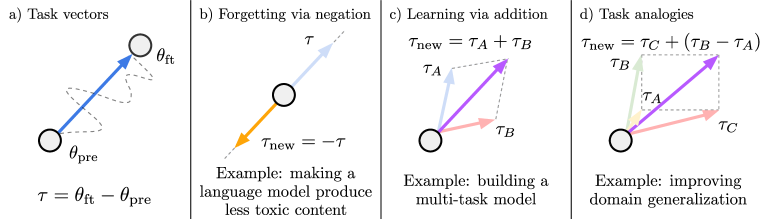
\includegraphics[width=0.84\paperwidth,height=0.50\paperheight,keepaspectratio]{images/llm-rlhf/merging_task_vector_arithmetic.png}
    \caption*{\scriptsize Ilharco et al., ``Editing Models with Task Arithmetic,'' ICLR 2023, \href{https://arxiv.org/abs/2212.04089v3}{arXiv:2212.04089v3}, Figure~1.}
  \end{figure}
\end{frame}

\begin{frame}[t,allowframebreaks]{Merging Recipes}
  \begin{itemize}\itemsep0.35em
    \item[\textcolor{red}{$\blacktriangleright$}] \textbf{Linear (model soup):} a weighted average of the checkpoints. Cheap, and the baseline every other method is measured against.
    \item[\textcolor{red}{$\blacktriangleright$}] \textbf{SLERP:} interpolate along the geodesic rather than the chord, which avoids the drift toward the origin that straight-line averaging causes. Defined for two parents at a time.
    \item[\textcolor{red}{$\blacktriangleright$}] \textbf{TIES} (Yadav et al., 2023) attacks the two ways task vectors interfere (redundant entries, and sign disagreement) in three steps:
      \begin{itemize}
        \item \textbf{Trim:} keep only the top 20\% of each $\tau$ by magnitude, reset the rest to zero.
        \item \textbf{Elect sign:} for each parameter, pick the sign whose total magnitude across models is larger.
        \item \textbf{Disjoint merge:} average \emph{only} the entries whose sign matches the elected one, leaving the zeros out of the denominator.
      \end{itemize}
    \item[\textcolor{red}{$\blacktriangleright$}] \textbf{DARE} (Yu et al., 2024) is a preprocessing step, not a merge: \textbf{d}rop delta parameters at rate $p$ \textbf{a}nd \textbf{re}scale the survivors by $1/(1-p)$, so the expected update is unchanged. Dropping 90\% of an SFT delta, and 99\% on the largest models, costs little accuracy. It works only because those deltas are tiny; continued pre-training grows them and the method stops working. Note what is dropped: the \emph{delta}, never the merged weight.
    \item[\textcolor{red}{$\blacktriangleright$}] \textbf{mergekit} (Goddard et al., 2024) implements all of these behind one config file, so trying a recipe costs minutes.
  \end{itemize}
\end{frame}

\begin{frame}{TIES-Merging: Trim, Elect Sign, Merge}
  \begin{figure}
    \centering
    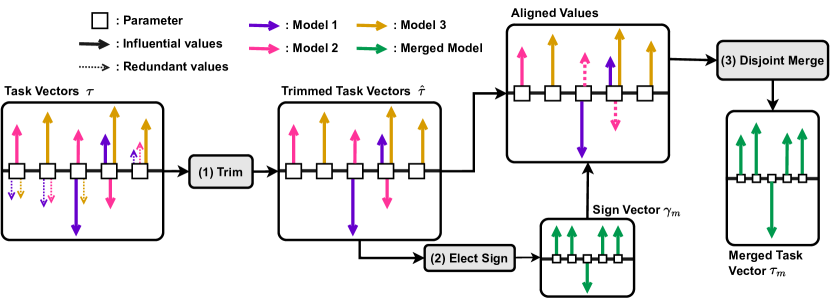
\includegraphics[width=0.86\paperwidth,height=0.52\paperheight,keepaspectratio]{images/llm-rlhf/merging_ties_pipeline.png}
    \caption*{\scriptsize Yadav, Tam, Choshen, Raffel \& Bansal, ``TIES-Merging: Resolving Interference When Merging Models,'' NeurIPS 2023, \href{https://arxiv.org/abs/2306.01708v2}{arXiv:2306.01708v2}, Figure~1.}
  \end{figure}
\end{frame}

\begin{frame}[t]{Merging LoRA Adapters, and When It Fails}
  \begin{itemize}\itemsep0.45em
    \item[\textcolor{red}{$\blacktriangleright$}] A LoRA adapter is \emph{already} a task vector: $\tau = \tfrac{\alpha}{r}BA$. Fold each adapter into the base and merge the results, and every recipe above applies unchanged.
    \item[\textcolor{red}{$\blacktriangleright$}] \textbf{Do not average $A$ and $B$ separately.} The product is bilinear, so
      $\tfrac{1}{2}(B_1 + B_2)\tfrac{1}{2}(A_1 + A_2) \neq \tfrac{1}{2}(B_1A_1 + B_2A_2)$;
      the cross terms $B_1A_2$ and $B_2A_1$ are noise neither adapter ever trained. Merge in $\Delta W$ space, or concatenate the factors and let the rank grow.
    \item[\textcolor{red}{$\blacktriangleright$}] \textbf{Merging is only defined between homologous models:} the same architecture from the same pre-trained checkpoint. Two models with the same shape but different pre-training have no shared coordinate system, and the average is nonsense.
    \item[\textcolor{red}{$\blacktriangleright$}] \textbf{The failure mode is silent.} A bad merge still loads, still generates fluent text, and still scores respectably on the benchmarks the parents were good at. Safety behaviour and instruction-following degrade first and are exactly what a quick eval will not catch. Evaluate the merge, never the recipe.
  \end{itemize}
\end{frame}

\begin{frame}[t,allowframebreaks]{Continual Learning for Deployed Models}
  \begin{itemize}\itemsep0.4em
    \item[\textcolor{red}{$\blacktriangleright$}] A deployed model is never finished: new domains, new products, new policy. Retraining from scratch each time is unaffordable, and tuning on only the new data causes \textbf{catastrophic forgetting}: the update overwrites weights the old capabilities depended on.
    \item[\textcolor{red}{$\blacktriangleright$}] \textbf{Replay.} Mix a slice of the original training data back into every new run. The simplest defence, and usually the most effective one.
    \item[\textcolor{red}{$\blacktriangleright$}] \textbf{Regularisation.} Penalise movement in the directions that mattered before. \emph{Elastic weight consolidation} (Kirkpatrick et al., 2017) weights that penalty per parameter by the Fisher information of the old task.
    \item[\textcolor{red}{$\blacktriangleright$}] \textbf{Constrain the update.} Biderman et al.\ (2024) found LoRA learns \emph{less} than full fine-tuning on code, and by a smaller margin on maths, because full fine-tuning finds updates of 10 to 100 times the rank. It also forgets less, holding the base model's behaviour outside the target domain better than weight decay or dropout do.
    \item[\textcolor{red}{$\blacktriangleright$}] \textbf{Merge instead of retrain.} Keep the deployed model, train the new capability separately, and merge. You get a rollback path: the parents are still on disk.
  \end{itemize}
\end{frame}
